\section{脅威モデル}
\label{sec:threat-model}
本章では,はじめにDNSの概要について述べる.
その次に,本研究における脅威モデルであるDNSトンネリングについて説明する.

\subsection{DNSの概要}
\label{sec:dns-protocol}

DNSは,ドメイン名に関連づけられたリソースレコードを解決するシステムである~\cite{rfc1034, rfc1035}.
DNSがユーザから問い合わせられたドメイン名のIPアドレスを解決することで,ユーザは識別しづらいIPアドレス(IPv4:``93.184.216.34", IPv6:``2606:2800:220:1:248:1893:25c8:1946")を直接入力することなく,サーバにアクセスすることができる.
このような利便性を実現するDNSによる名前解決の機能は,ユーザがインターネットを利活用する上で極めて重要である.

\subsubsection{名前空間}
DNSにおける名前空間は,委譲の仕組みに基づいて,ルートのゾーンを頂点に上位のドメインが下位のドメインにゾーンを分けていくことによって階層的に分割された構成になっている.
ドメイン名では,右から左方向に階層の序列が表現されている.
例として,``example.com"を考える.
ルートドメインは一般に省略され,TLD(Top Level Domain)と呼ばれるルートの1つ下の階層に位置づくドメインは,この場合``com"である.
階層間の区切りには,ドット(``.")が使用される.
TLDの1つ下に位置づくSLD(Second Level Domain)は,この場合``example"である.
それぞれの名前空間はゾーンと呼ばれ,上位のドメインがその下位ドメインにゾーンを委譲することによって分割される.
委譲の仕組みによってドメインごとにゾーンが分割されるのは,図~\ref{fig:dns-architecture}の色で区別する通りである.
このゾーンは権威サーバによって管理され,権威サーバはゾーンファイルにドメイン名とレコードデータを記述することでドメイン名にレコードデータを関連づけることができる.
委譲に基づいたゾーン分割の仕組みは,初期のDNSにおけるRoot.hintsを用いた中央集権的な管理に伴うデータの同期の課題に対処したものである.
Root.hintsによる単一ファイルによる管理では,増加するドメイン名に対応することが困難であった.
委譲の仕組みによって,管理するドメイン名の対象をゾーンで分割されるため,負荷分散が実現されている.

\begin{figure}[th]
 \centering
 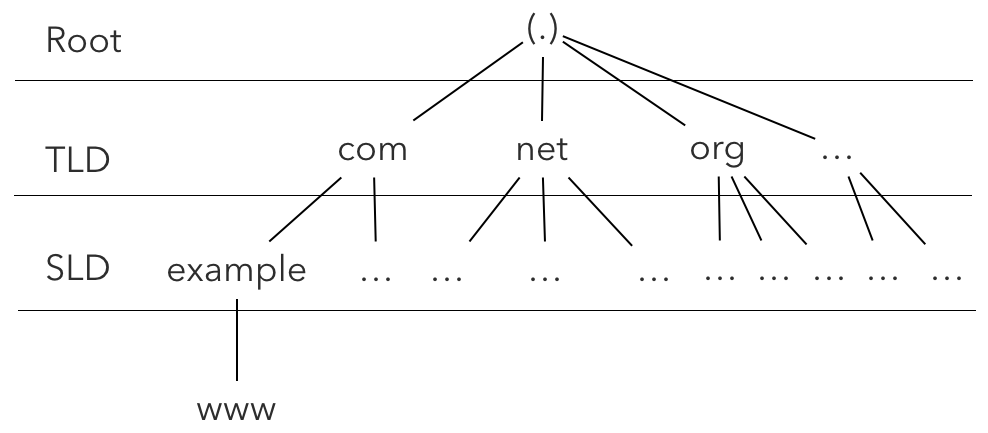
\includegraphics[width=12.0cm]{figure/dns-architecture.png}
 \caption[ゾーンごとに分割された名前空間]{ゾーンごとに名前空間を色で区分した様子.Root権威が管理するオレンジで表現されたゾーンには,comやorgをはじめとしたドメインが含まれる.Rootの直下に位置するTLDの一つであるcomドメインは,青色で囲まれたexampleドメインを含むゾーンを管理する.comに紐づけられるexampleドメインは,wwwなどを管理する.}
 \label{fig:dns-architecture}
\end{figure}

\textbf{アーキテクチャ}\\
DNSは,クライアント・サーバアーキテクチャで構成され,機能に基づき3つのサービスに分類することができる.
\begin{itemize}
 \item スタブリゾルバ
 \vspace{-3mm}
 \item フルサービスリゾルバ
 \vspace{-3mm}
 \item 権威サーバ
\end{itemize}

スタブリゾルバは,名前解決の問い合わせを行うクライアントノードである.
フルサービスリゾルバ(キャッシュサーバやリカーシブサーバとも呼称される)は,スタブリゾルバに代わって,リソースレコードを保持する権威サーバに問い合わせるクライアントノードである.
名前解決をする際には,ルートから順にTLD,SLDという具合に権威サーバに再帰的に問い合わせることで,最終的に目的のドメイン名に関するリソースレコード情報を取得する.
この時,はじめのルート権威サーバのアドレスは``Root.hints"と呼ばれるファイルに基づいて問い合わせるが,それより下位のドメインについては,上位の権威サーバが次の権威サーバのアドレスを応答することで名前解決のチェーンを繋げている.
すなわち,ルート権威サーバがTLDの権威サーバのアドレスを応答し,TLDの権威サーバがSLDの権威サーバのアドレスを応答していく具合である.
権威サーバは,リソースレコードを保持するサーバノードであり,フルサービスリゾルバからの問い合わせ依頼に応答する.

\subsubsection{ドメイン名とリソースレコード}
\label{sec:domain-resorce-record}
%TLDごとに登録するプロセスや必要書類,金額は異なり,上位
ルートからホストまでの階層構造の繋がりは,``label3.label2.label1."のように右から左方向に連結することで表現される.
この表記は,FQDN(Fully Qualified Domain Name)と呼ばれ,右端のドットがルート,``label1"がTLD,``label2"がSLDを表現し,ドメインごとの階層にはドットが使用される.
ドメインの階層構造において,全てはルートを頂点としているため,ルートを意味するドットを略記した``label3.label2.label1"が,一般にはドメイン名として解釈される.
次にドメイン名に関する長さおよび使用できる文字列について説明する.
\vspace{-1pt}
\begin{eqnarray}
 (LabelD).(LabelC).(LabelB).(LabelA). \label{eq:domain-name} \\
 (Length) + (LabelD) + ... + (length) + (LabelB) + (length) + (LabelA) + 0 \label{eq:label-name} \\ 
 1 + (Max 63) + ... + 1 + (Max 63) + 1 + (Max 63) + 1 = (Max 255) \label{eq:length-label-domain}
\end{eqnarray}

(\ref{eq:domain-name})は,複数のラベルで構成されたドメイン名の例である.
(\ref{eq:label-name})は,Questionヘッダーに注入される際のそのドメイン名を表すデータである.
Questionセクションでは,ドメイン名を表す際にドットは省略され,ラベルの長さとラベル名,そしてドメイン名の終わりを意味する``0"で表現される.
(\ref{eq:length-label-domain})は,ラベルの長さとラベル名のサイズを表す.
ラベルの長さは,1バイトのサイズで表現され,ラベル自体の最大長は63バイトである.
Questionセクションの最大長255バイトは,ラベルの長さとラベル,そしてドメイン終了を表す``0"を含めた長さである.
このため,最初のラベル長を表す1バイトとドメイン名の終了を意味する``0"を表すための1バイトを差し引いた253バイトが,実際のドメイン長の最大長である.

ラベルには,数字とアルファベットおよびハイフン(``-")を使用することができ,ラベル中に大文字・小文字の区別はない.
他方で,アルファベットなどのASCII以外にも,国際化ドメイン名(IDN: Internationalized Domain Name)を使用すると日本語やアラビア語なども使用することができる.
IDNは,Punnycode\footnote{Punnycode: Unicode文字列を一意かつ可逆的にASCII文字列に変換する符号化方式.}などのエンコーディング手法に基づき,DNSクエリする際にはASCIIコードに変換される~\cite{idn}.

\begin{table}[htb]
 \centering
  \begin{tabular}{ccc}
    \toprule
		\textbf{タイプ} & \textbf{値} & \textbf{意味} \\
    \midrule
    A & 1 &  ホストのIPv4アドレス \\
    NS & 2 & 権威サーバ \\
    MF & 4 & メール転送サーバ \\
    CNAME & 5 & 別名 \\
    SOA & 6 & 権威ゾーンの開始 \\
    NULL & 10 & NULL(実験用) \\
    PTR & 12 & ドメイン名のポインター(逆引き) \\
    HINFO & 13 & ホスト情報 \\
    MINFO & 14 & メールボックスおよびメールリスト情報 \\
    MX & 15 & メール交換 \\
    TXT & 16 & 任意文字列 \\
    \bottomrule
  \end{tabular}
 \caption{主要リソースレコード一覧}
 \label{tab:resource-record}
\end{table}

\newpage
ドメイン名に関連づけられる情報はリソースレコードと呼ばれ,目的に応じて複数のタイプが定義されている.
例えば,ドメイン名にIPv4アドレスを関連づけることを考える.
そのドメインの権威サーバは,関連づけたいIPv4アドレスをレコードタイプAとして,ゾーンファイルに記述する.
クライアントは,ドメイン名とレコードタイプとしてAを指定しサーバに問い合わせることで,権威サーバが事前に登録したAレコードに記述されたアドレスを取得することができる.
DNSでは,IPv4アドレス以外にも様々な情報をドメイン名に関連づけることができる.
代表的なソースレコードのタイプを表~\ref{tab:resource-record}で示す.

\begin{table}[htbp]
	\caption{DNSのパケットフォーマット}
	\centering
   \scalebox{1.5}{
	 \begin{tabular}{|l|}
		\hline
		 Header\\ \hline
		 Question\\ \hline
		 Answer\\ \hline
		 Authority\\ \hline
		 Additional\\ \hline
	 \end{tabular}
   }
	\label{tab:packet-format}
 \end{table}

次に,DNSのパケットフォーマットについて説明する.
表~\ref{tab:packet-format}で示すように,DNSのパケットは5つのセクションに分けられる.
%\begin{figure}[bh]
% \centering
% 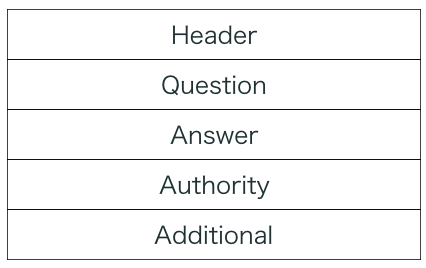
\includegraphics[scale=0.7]{figure/dns-format.png}
% \caption{DNSのパケットフォーマット}
% \label{fig:dns-format}
%\end{figure}
クライアントがDNSの名前解決をする際,解決したいレコードタイプとそのドメイン名は表~\ref{tab:answer-dns}におけるNameフィールドに格納される.
各フィールドはサイズが決まっており,Qnameフィールドが最大長255バイト,リソースレコードのタイプを表すQtypeフィールドとクエリクラスを表すQClassフィールドがそれぞれ2バイトとなっている.
RDLengthは,応答データが含まれるRDataの長さが格納される.
\begin{table}[htbp]
 \caption{DNSのAnswerセクション(bits)}
 \centering
  \begin{tabular}{|c|c|c|c|c|c|}
    \toprule
		%\multicolumn{6}{|c|}{(bits)}\\
    %\midrule
		Name & Type & QClass & TTL & RDLength & RData\\
		(可変長) & (16) & (16) & (32) & (16) & (可変長)\\
    \bottomrule
  \end{tabular}
 \label{tab:answer-dns}
\end{table}

%\begin{figure}[th]
% \centering
% 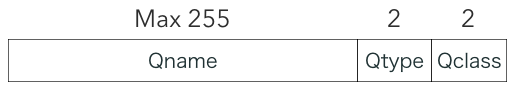
\includegraphics[scale=0.6]{figure/dns-answer.png}
% \caption{DNSのパケットのAnswerセクション(bytes)}
% \label{fig:dns-answer}
%\end{figure}

\subsubsection{名前解決の仕組み}
\label{sec:dns-mechanism}

例えば,クライアントが``www.example.com"のIPv4アドレスを解決する場合を考える.
はじめに,クライアントとなるスタブリゾルバは,スタブリゾルバと同一セグメント内のフルサービスリゾルバもしくは,ネットワークセグメントに依らないどこからでもアクセスできるフルサービスリゾルバ(オープンリゾルバ,パブリックリゾルバとも呼称される)に問い合わせる.
フルサービスリゾルバは,その名前解決クエリが過去に解決したものでないかキャッシュデータを確認する.
キャッシュにヒットした場合にはキャッシュの情報をクライアントに応答され,ヒットしなかった場合には,root.hintsファイルを参照しルート権威サーバにリクエストパケットを転送する.
クエリ(問い合わせ)を受け取ったルート権威サーバは,``com"ドメインを委譲した権威サーバのアドレスを応答する.
次に,フルサービスリゾルバは,``com"の権威サーバに対し同じクエリを転送する.
``com"の権威サーバは,``example.com"ドメインを委譲した権威サーバのアドレスを応答する.
フルリゾルバは,``example.com"の権威サーバに同じクエリを転送する.
``example.com"の権威サーバは,保持するゾーンファイルからクエリされたドメインのリソースレコードについて探索し,探索の結果としてレコード情報をフルサービスリゾルバに応答する.
フルサービスリゾルバは,権威サーバから応答された情報をスタブリゾルバに転送することで,問い合わせられた名前は解決される.
DNSによる名前解決の一連の動作を図~\ref{fig:dns-name-resolution}で示す.
\begin{figure}[htbp]
 \centering
 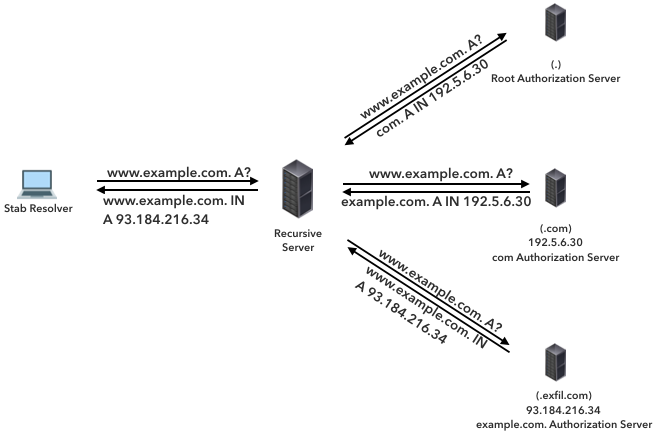
\includegraphics[width=12.0cm]{figure/dns-name-resolution.png}
 \caption{DNSによる名前解決}
 \label{fig:dns-name-resolution}
\end{figure}


%リソースレコードのタイプごとの使用頻度を知りたい
% タイプごとの説明を充実させるのは,重要かもしれない


\newpage
\subsection{DNSトンネリング}
\label{sec:dns-tunneling}
%DNSトンネリングが脅威となりうる点に関する説明
%Botnetなどに使用されることについて言及するべき
%概念
現在,情報流出を目的とするマルウェアのほとんどは,秘匿通信手法を利用しているとされている~\cite{asaf}.
DNSトンネリングは,そのような秘匿通信の代表的な手法である.
DNSトンネリングという名称は,DNSをデータ転送のメディアとした秘匿通信手法の総称であり,転送元と転送先の方向に基づき2つに分類することができる.
一方がスタブリゾルバから権威サーバへのデータ転送手法であるDNS Exfiltration,他方が権威サーバからスタブリゾルバへのデータ転送手法がDNS Infitrationである.
%DNSトンネリングという手法は,ポートスキャンで知られるNmapのメーリングリストだとされている.
以下に示すDNSの特性を利用することによって,DNSトンネリングは機能する.

\begin{itemize}
 \setlength{\itemsep}{0pt}
 \item パケットフォーマットの構造において,任意の文字列を注入できるフィールドを保持する
 \item 名前解決の通信はほとんどのサービスに先立って発生するため,
	\begin{itemize}
	 \vspace{-10pt}
   \setlength{\itemsep}{0pt}
	 \item DNSのサービスポートが開かれ,フィルタリングされることが少ない
	 \item トラフィックが肥大化しやすく,長期でログを管理すること少ない
	\end{itemize}
\end{itemize}

DNSトンネリングがデータ転送のキャリアとするフィールドは,クエリのQuestionセクションのQnameと,AnswerセクションのRdataである.
QuestionセクションのQnameフィールドを利用することで,スタブリゾルバから権威サーバ方向にデータを転送できる.
この方向の通信は,ビーコン通信やターゲットから取得した情報を外部に漏えいさせるといった攻撃の最終目的を達成するのに使われる.
また,AnswerセクションのRdataフィールドを利用することで,データを転送することができる.
この通信は,ターゲットネットワーク内のホストに潜伏したマルウェアなどへの命令コードを送信するのに使われる.
さらに,この二つのキャリアを利用することが双方向の通信路を確保できるため,C2通信を実施することも可能である.
%DNSトンネリング手法が脅威なのは,IDS・IPSなどの検知システムにフィルタリングされにくく,クエリ頻度を長期化させた場合解析を迂回することができる点である.

DNSトンネリング手法が初めて一般に公開されたのは,1998年に,ポートスキャンで知られるNmapのメーリングリストだとされている~\cite{nmap, maarten}.
2004年には,Dan KaminskyがOzymanDNS~\cite{ozymandns}と呼ばれるDNSトンネリングの実装を公開した~\cite{dan-kaminsky}ことをきっかけに広く知られるようになった.
それ以降,数多くのDNSトンネリングの実装~\cite{heyoka, iodine, dnscat2, tcp-over-dns, dnscat, denise, dns-shell, dnsbotnet, dnscapy, dohtunnel, godoh, dohc2, magictunnelandroid, dns2tcp, tuns}が公開され,実際のサイバー攻撃に悪用されるようになっている.

\subsubsection{DNS Exfiltration}
\label{sec:dns-exfiltration}
% トンネリング実装のUpstreamは,どのくらいなのだろうか

本項では,スタブリゾルバから権威サーバ方向にデータを転送する手法であるDNS Exfiltrationの詳細について説明する.
DNS Exfiltrationは,名前解決として問い合わせられるドメイン名が,そのドメインのゾーンを管理する権威サーバに転送される仕組みを利用した手法である.
DNSでは,ドメイン名に関連づけられるリソースレコードの情報は,そのドメインをゾーンとする権威サーバが保持しており,ルートから再帰的に問い合わせていくことでその権威サーバからの応答を受け取る.
このため,問い合わせられたドメイン名が実在しない場合でも,再帰問い合わせの仕組みに従って,そのドメイン名の最後の権威サーバまで転送されることになる.
権威サーバでは通常,クエリされたドメイン名の実在性の有無に依らず,問い合わせられたクエリ情報をログとして管理する.
このような特性に踏まえてDNSを利用すると,DNSクエリのドメイン名のラベルに組織外ネットワークに転送したい文字列を注入することで,組織外ネットワーク上に設置された権威サーバにそのデータを転送することができる.
これがDNS Exfiltrationの動作原理である.

このような仕組みのDNS Exfiltrationを動作させるには,宛先となる権威サーバを用意する必要があり,グローバルなドメインを取得することを前提としている.
第~\ref{sec:dns-mechanism}項で述べるように,ドメイン名の最大長は253バイトであり,その内ラベルの最大長は63バイトという制約がある.
そのため,DNS Exfiltration手法を用いてデータを転送する際には,TLDのラベルと宛先権威サーバのラベルもしくはSLDラベルと権威サーバのラベルを差し引いたサイズが実際に転送できる最大長となる.
また,任意の文字列をDNS Exfiltrationメソッドを用いて外部に転送するにあたり,転送キャリアであるドメイン名における文字列制約を満たすように転送したいデータに前処理を施す必要がある.
ドメイン名に使用できる文字列は,第~\ref{sec:dns-mechanism}項で述べるように,``a"から``z"までのアルファベットと``0"から``9"までの数字と先頭以外のハイフン``-"記号である.
この文字列制約については,転送したいデータをバイナリデータに変換し,そのバイナリデータをラベルとして印字可能なASCIIコードに変換することでその制約を満たすことができる.
この前処理について,既存のDNSトンネリング実装の多くがBase Encodingを用いている~\cite{rfc4648}.
%使用するエンコーディング手法によって,データの圧縮率は異なる.
この処理によって,転送データがバイナリデータである際にも転送効率上げたり,ラベルの文字列制約を満たさないデータも転送することができる.
また,エンコーディングのラベルは,自然言語とは異なるため,メッセージの意味抽出を困難にすることにも機能する.

ここで,DNS Exfiltrationを用いて,あるイントラネット内のホストからイントラネット外のホストにデータを転送することを考える.
転送される宛先となるイントラネット外のホストには,``exfil.com"より下位の全ての名前空間をゾーンとする権威サーバ(``exfil.com")を指定する.
転送したい文字列にエンコーディング前処理を施した後,``用意した文字列.exfil.com"という具合に文字列をラベルとして含めることで,ドメイン名が用意できる.
適当なリソースレコードタイプを指定し,DNSクエリとして転送すると,その権威サーバにはログとして,文字列を含んだドメイン名を取得する.
最後に,受け取ったサーバサイドは,前処理と逆のデコード処理を施すことで,オリジナルのデータを取得できる.
以上のように再帰問い合わせとラベルという転送キャリア,エンコーディング処理を組み合わせることで,イントラネット内のホストから外部ネットワークに任意の情報を転送することができる.
これが,DNS Exfiltrationの動作メカニズムである.
DNS Exfiltrationのメカニズムは,図~\ref{fig:dns-exfiltration}で示す通りである.
\begin{figure}[htbp]
 \centering
 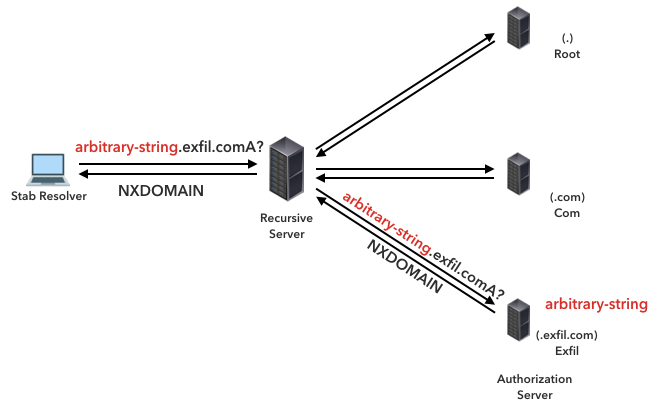
\includegraphics[scale=0.6]{figure/dns-exfiltration.png}
 \caption[DNS Exfiltrationの概略図]{ドメイン名のラベル部に任意の文字列が注入されたDNSクエリが,インターネット上の権威サーバ(``exfil.com")に転送される様子.}
 \label{fig:dns-exfiltration}
\end{figure}

%具体的な脅威モデル
%検知バイパス手法 : スループット(パフォーマンス)を下げることによる秘匿性,一般的なホスト名を使った対応表

%1998年4月,DNSトンネリングの手法は,NmapのBugtraqメーリングリストにて初めて公になったとされている\cite{bugtraq}.

\subsubsection{DNS Infiltration}
\label{sec:dns-infiltration}

本項では,権威サーバからスタブリゾルバ方向にデータを転送する手法であるDNS Infiltrationの詳細について説明する.
DNS Infiltrationは,DNSにおける幾つかのリソースレコードが任意の文字列を記述できる設計を利用したデータ転送手法である.
ドメイン名に関連づけられた情報を管理・提供する権威サーバは,ゾーンファイルに関連づけたい情報を記述する.
リソースレコードには,レコード情報を検証する機構が備わっていないため,任意の文字列を登録することができる.
特に,記法が決まっていないTXTタイプやNULLタイプなどもあり,DNS Infiltrationではこのようなレコードタイプに転送したいデータを登録しておく.
このようにして登録されたレコード情報について,名前解決問い合わせすることによって,インターネット(権威サーバ)からイントラネット(スタブリゾルバ)にデータを転送することができる.
DNS Infiltrationとして利用され得るレコードタイプについて,これまでのトンネリング実装で使用されたものに基づいてまとめたのが,表~\ref{tab:infil-rtype}である.
%zonefileを説明
%Infilとして使用される脅威のあるRtypeを列挙

\begin{table}[h]
 \centering
  \begin{tabular}{lrll}
    \toprule
		\textbf{タイプ} & \textbf{\begin{tabular}{c}最大サイズ\\(byte)\end{tabular}} & \textbf{説明} & 実装\\
    \midrule
		A & 4 & \ ホストのIPv4アドレス &\\ \hline
		NS & 4 & \ 権威サーバ & \ \cite{dnscat2}\\ \hline
    %MF & 4 & メール転送サーバ \\
		CNAME & 253 & \ 別名 & \ \cite{iodine},\cite{dnscat2}, \cite{dnscapy}, \cite{tuns}\\ \hline
		%SOA & 253 & 権威ゾーンの開始 & \\
		NULL & 255 & \ NULL(実験用) & \ \cite{iodine}\\ \hline
		PTR & 4 & \begin{tabular}{l}ドメイン名のポインター\\(逆引き)\end{tabular} & \\ \hline
    %HINFO & 13 & ホスト情報 \\
    %MINFO & 14 & メールボックスおよびメールリスト情報 \\
		MX & 253 & \ メール交換 & \ \cite{iodine},\cite{dnscat2}\\ \hline
		TXT & 255 & \ 任意文字列 & \begin{tabular}{l}\cite{iodine},\cite{dnscat2}, \cite{denise}, \cite{dns-shell},\\ \cite{dnscapy}, \cite{dohtunnel}, \cite{dohc2}\end{tabular}\\ \hline
		AAAA & 32 & \ ホストのIPv6アドレス & \\ \hline
		SRV & 180 & \begin{tabular}{l}ドメイン名に対する\\サービスの場所\end{tabular} & \ \cite{iodine}\\ \hline
		 DNSKEY & 40 & \ DNSSECのための公開鍵 & \ \cite{dns2tcp}\\
    %TLSA & 52 & \\
    \bottomrule
  \end{tabular}
 \caption{DNS Infiltrationのメソッドとして使用することができるレコードタイプの一覧}
 \label{tab:infil-rtype}
\end{table}


\newpage
NS・CNAME・MXレコードでは,DNS Exfiltrationと同じ要領でドメイン名のラベルに転送したい文字列を注入できる.
また,NULL・TXT\footnote{EDNS0を使用する場合,65,535bytesが最大長となる.}・SRV・DNSKEYを用いる場合には,レコード構文に指定がないため任意の文字列をそのまま注入できる.
最後に,A・AAAA・PTRレコードを用いる場合には,転送したい文字列を数字に変換させた後に,ドット(.)区切りもしくはコロン(:)区切りで注入できる.

\begin{eqnarray}
 www.exfil.com. \qquad IN \quad TXT \quad uname \ -ap
 \label{eq:infil-txt}
\end{eqnarray}
TXTレコードタイプを用いてDNS Infiltrationすることを考える.
(\ref{eq:infil-txt})は,TXTレコードを用いてホストで実行させるLinuxコマンドを転送する例である.
転送されるunameプログラムは,システム情報を取得するプログラムである.
実行結果をDNS Exfiltration手法を用いて転送することで,ホストマシンにおけるシステムのカーネルバージョンやプロセッサの種類などの情報を取得することができる.
次に,スタブリゾルバは,``www.exfil.com"の``TXT"レコードタイプを通常通り問い合わせる.
再帰問い合わせの仕組みに基づいて,そのDNSクエリは``exfil.com"まで転送され,ゾーンファイルのTXTレコードタイプの値がフルサービスリゾルバを経由したのち,スタブリゾルバまで応答される.
DNS Infiltrationの流入通信を図解した様子が,図~\ref{fig:dns-infiltration}である.
このようにして,DNS Infiltrationでは,正規の名前解決の方法を用いて,インターネットから組織内へとデータを取得することができる.
\begin{figure}[htbp]
 \centering
 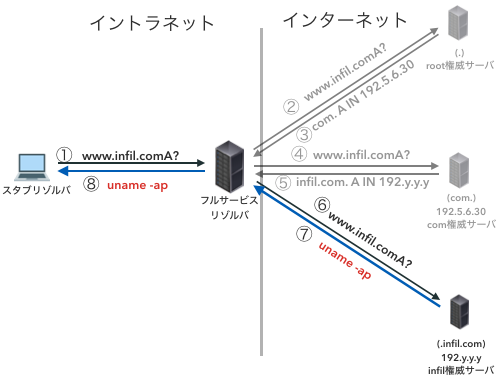
\includegraphics[scale=0.5]{figure/dns-infiltration.png}
 \caption[DNS Infiltrationの概略図]{TXTレコードに登録された情報について,DNSクエリで問い合わせることで権威サーバから命令情報を取得している様子}
 \label{fig:dns-infiltration}
\end{figure}


% Null タイプは,厳密に定義されておらず,実験用としか表現されていない.しかし,全体のタイプのうち,20%を示す程度に頻繁に使用されるタイプのである.

\newpage
\subsection{DNSトンネリングへの既存対策}

本節では,DNSトンネリングに対するこれまでの対策手法を紹介し,検知手法として用いられるアプローチについて説明する.
最後に,それら検知アプローチを迂回する脅威モデルを示し,検知に基づくアプローチに限界があることを明らかにする.

DNSトンネリングに対して,森下ら~\cite{morishita}は提案されているDNSトンネリングへの対策アプローチを以下のようにまとめている.
\begin{enumerate}
 \item DNSクエリログの取得と保存・内容の調査
 \vspace{-0.5cm}
 \item エンタープライズネットワークにおけるOP53B\footnote{OP53B : 組織外に設置されたオープンリゾルバのようなフルサービスリゾルバや権威サーバとの通信を抑止するために,組織外ネットワークを宛先とする53番ポートの通信をブロックする仕組み.}の適用
 \vspace{-0.5cm}
 \item DNSファイヤーウォールの導入
\end{enumerate}
クエリログの取得は解析・調査のために必要不可欠である一方で,DNSのログファイルは肥大化しやすく管理コストが課題になる.
OP53Bの適用は,組織内部からの名前解決トラフィックをイントラネットに設置されたフルサービスリゾルバに集約することができるため,オープンリゾルバならびに権威サーバと直接通信することに伴う悪性通信の発生抑止に寄与する.
DNSファイヤーウォールとは,ベンダーが独自に開発したトンネリングなどの悪性通信の統計データから閾値や機械学習モデルに基づき,悪性トラフィックを検知・ブロックする製品を指す.

% 検知に基づく手法の現在までの程度を淡々と示す.
%誰がその特徴を発見したのか
%それ特徴を用いて,どのようなテクニックで検知手法として確立させたのか
\subsubsection{特徴量}
\label{sec:pre-tunnel-feature}
従来,DNSトンネリング通信の検知には,以下に示す特徴量について統計分析を用いた閾値の算出や機械学習を用いた悪性モデルが用いられてきた.
トンネリング実装などによって発生する一般的なDNSトンネリング通信の検知にあたり,以下のような特徴を利用した手法がこれまでに多数提案されている.\newline
%長さ
%DNS Exfiltrationでは,Qnameフィールドのラベルがデータ転送のキャリアとなるため,表~\ref{tab:feature-tunnel}で示すように,転送するデータ量に比例してドメイン名は長くなる.
%また,DNS Infiltrationの場合は,応答パケットのRdataフィールドがデータ転送のキャリアとなるため,転送するデータ量に比例して肥大化する.


\hspace{-12pt}\textbf{ドメイン名の長さとクエリパケットのサイズ}\\
\hspace{12pt}クライアントからサーバ方向にデータを転送させるDNS Exfiltration手法において,転送キャリアとなるドメイン名が注入されるデータ量に応じて長くなる~\cite{vern}.
例えば,DNS Exfiltrationにおいて,一回あたりのデータ転送量を増加させる場合,Qnameフィールドのドメイン長もそれに比例して長くなり,結果としてパケットサイズも増加するという具合である.
DNS Infiltrationにおいても同様で,一回あたりのデータ転送量を増加させる場合,Rdataフィールド内のデータ量も大きくなり,応答パケットのサイズが増加する.

\begin{table}[th]
 \caption{正規DNSクエリとDNSトンネリングにおけるドメイン名の違い}
 \centering
  \begin{tabular}{l|l}
    \toprule
		\multicolumn{1}{c}{\textbf{種類}} & \multicolumn{1}{c}{\textbf{ドメイン名}} \\
    \midrule
    正規 &  www.example.com \\ \hline
    トンネリング & arbitrary-long-text-utill-it-reaches-253byte.example.com\\
    \bottomrule
  \end{tabular}
 \label{tab:feature-tunnel}
\end{table}


%同一ドメインあたりのクエリ頻度
\hspace{-12pt}\textbf{同一ドメインあたりのトラフィック頻度}\\
\hspace{12pt}DNSトンネリングでは,一度に転送できるデータ量に限界があるため,目的のデータを全て転送するには分割する必要がある.
トンネリング実装のように対話的にシェルコマンドを実行する通信の場合,トラフィック頻度は極めて高頻度になる.
また,サイズの大きいデータをDNS Exfiltrationを用いて転送する場合も同様に,複数のパケットに分割されたデータを転送するにあたって,多数のトラフィックが発生することになる.\newline

%レコードタイプ
\hspace{-12pt}\textbf{リソースレコードのタイプ}\\
\hspace{12pt}理論的に全てのリソースレコードを用いてデータを転送することは可能であるが,第~\ref{sec:dns-infiltration}項で示すように,使用するレコードタイプによって転送できるデータ量は大きく異なる.
表~\ref{tab:infil-rtype}で示すように,実際のトンネリング実装におけるDNS Infiltrationを目的とする通信では,AやAAAAなどは使われず,CNAMEやTXTが主に使用される.
AやAAAAなどのレコードタイプが使用されない背景には,数字のみの文字列制約が厳しさと最大のデータサイズに小さいことが考えられる.
TXTの最大サイズが253bytesであるのに対して,Aが4bytesでAAAAが32bytesなのは明らかに小さいことが確認できる.
他方で,通常のインターネットの利活用において使用されるレコードタイプに極端な分布の偏りがあることが知られている.
Herrymannら~\cite{Herrymann}は,~2010年~1月~1日から~6月~30日までの期間において,大学構内に設置されたフルサービスリゾルバによるDNSログデータを収集した.
収集の結果,ドメイン名に対するIPv4とIPv6のアドレス解決の通信が全体の大部分の89.407\%を占め,Infiltrationとして使用されるCNAMEやTXTは~1\%に満たないことが明らかになった(表~\ref{tab:distribution-rtype}).
以上のことから,TXTやCNAMEといった任意の文字列を注入できる反面,使用頻度が低いレコードタイプである特性から,データ転送効率と秘匿性がトレードオフであることが確認できる.
%レコードタイプは効率的なデータ転送を実現できる反面,


%これは,新規登録のドメイン名のみしか対応していないようだ
%Tatangら~\cite{tatang}が,2017年7月30日から9月1日までの期間にて,DNSサーバ間の通信パッシブDNS
%
%\begin{table}[h]
 \caption[リソースレコードの分布]{2017年7月から8月までのDNSトラフィックデータセットにおけるリソースレコードのタイプ分布}
 \centering
  \begin{tabular}{lrr}
    \toprule
    \textbf{タイプ} & \textbf{パケット数} & \textbf{割合(\%)}\\
    \midrule
    A & 1,121,025,638 & 54.90\\
    AAAA & 197,388,865 & 9.67\\
    MX & 682,948 & 00.3\\
    NS & 7,662,147 & 0.38 \\
    CNAME & 156,708,021 & 7.68 \\
    TXT & 41,593,164 & 2.04 \\
    NULL & 432,232,574 & 21.17 \\
    Other & 84,371,709 & 4.13 \\
    \bottomrule
  \end{tabular}
 \label{tab:infil-rtype}
\end{table}

%による調査では,表~\ref{tab:distribution-rr}で示す通り
\newpage
\hspace{-12pt}\textbf{パケットの応答ステータス}\\
\hspace{12pt}DNSのヘッダーは,表~\ref{tab:header-dns}で示すようなフィールドを持っており,問い合わせに対して,表~\ref{tab:dns-rcode}のようなステータス情報を応答する.
第~\ref{sec:bypass-method}項で示すような検知迂回手法を使う場合を除いて,
通常のDNS Exfiltrationでは,権威サーバが未知のデータがクラアントから転送される.
そのため,クライアントからの問い合わせには,コンテンツ不在を意味する``NXDomain"が応答される.
応答パケットのステータスが``NXDomain"であるとき,DNS Exfiltrationの可能性がある.
%表に書き換えることが可能である
%\begin{figure}[h]
% \centering
% 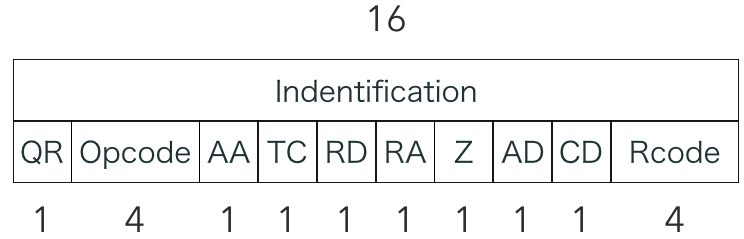
\includegraphics[width=10.0cm]{figure/dns-header.png}
% \caption{DNSのヘッダー(bytes)}
% \label{fig:dns-header}
%\end{figure}
%\vspace{-1cm}
\begin{table}[htbp]
 \caption{DNSのHeaderセクション}
 \centering
  \begin{tabular}{|c|c|c|c|c|c|c|c|c|c|}
    \toprule
		\multicolumn{10}{|c|}{Identification(16bits)}\\
    \midrule
		QR & Opcode & AA & TC & RD & RA & Z & AD & CD & Rcode \\
		(1) & (4) & (1) & (1) & (1) & (1) & (1) & (1) & (1) & (4) \\
    \bottomrule
  \end{tabular}
 \label{tab:header-dns}
\end{table}

\begin{table}[h]
 \caption{代表的なRcode一覧}
 \centering
  \begin{tabular}{rll}
    \toprule
		\multicolumn{1}{c}{\textbf{値}} & \multicolumn{1}{c}{\textbf{名前}} & \multicolumn{1}{c}{\textbf{意味}}\\
    \midrule
    0 & NoError & 正常\\
    1 & FormErr & フォーマットエラー\\
    2 & ServFail & サーバエラー\\
    3 & NXDomain & 存在しないドメイン\\
    4 & NotImp & 未実装\\
    5 & Refused & 問い合わせ拒否\\
    \bottomrule
  \end{tabular}
 \label{tab:dns-rcode}
\end{table}


%Qnameにおける文字列分布とエントロピー
% 結局Baseエンコーディングは,単に文字列をマッピングさせているだけなので,一方向性ではないので,オリジナルの文字列の分布と変化はない.
\hspace{-12pt}\textbf{ドメイン名に含まれる文字列の出現頻度}\\
\hspace{12pt}Bornら~\cite{born}は,ドメイン名に使用されている文字列の分布について,流布しているトンネリング実装と正規のDNS通信について調査した.
その結果,正規のドメイン名が英語における文字列の出現分布と相関があるのに対して,トンネリング実装によって生成されるドメイン名における文字列の出現頻度では相関がみられず,文字列の出現頻度はランダムとなる傾向にある.

%どのようめ手法を用いて,DNSトンネリング検知に取り組んできたのかを説明し,次の検知迂回手法の足がかりにする
%例えば,クラスタリングなのか,機械学習なのか,統計的な手法なのか
%ツール依存であり汎用性がないことを述べたい
%これまでに提案されてきたDNSトンネリングの検知手法は,第~\ref{sec:pre-tunnel-feature}項で述べるような特徴量に基づいている.

%全セクションで述べられるような検知手法を迂回する手法を述べ,既存の検知手法の限界を示し,アーキテクチャの変更の必要性を論じる
\subsubsection{既存検知手法に対する脅威モデル}
\label{sec:bypass-method}
%パフォーマンスを下げる手法(Low Latency)
%DNSエイリアスに対応づける手法
% 慣習的に命名されるラベル(Naming Convention)に意味を持たせることによって,例えば1byteの情報を持たせること
%特別Alexaなどの人気ラベルを調査しなくてもいいのかもしれない
% DoHを利用した手法もある
% 既存研究における課題として,ツール限定型の手法では汎用性がない
% しかし,これまでに提案されてきた手法は,Low throughput手法に対して十分ではない機能しない可能性がある
% 断定した方がいい,ファクトに基づいて議論しよう
% 99%まで検知することができているため,十分に有効な手段である,とか
% トンネリング対策として求められる要素の1つに,リアルタイム性があると思われる.
% リアルタイム検知では,トラフィック特徴を利用することが困難であるため,ペイロード特徴に頼るほかなく,検知することが困難である
本項では,既存検知アプローチを迂回する脅威モデルを示しながら,既存対策手法の課題を説明する.
% 既存検知手法の課題
第~\ref{sec:pre-tunnel-feature}項で示すように,DNSトンネリング手法に基づいてデータを転送するとき,正規のDNSクエリパケットと比べて,そのパケットは不自然に長くランダムなQnameになる性質や頻繁なトラフィックが発生するという性質が現れる傾向にある.
そのような性質を特徴量として分析することによって,これまでに多数の検知手法が提案されてきた~\cite{born, cheng, liu, asaf, steadman, jawad}.
その際,実際の攻撃シーンに使用されているDNSトンネリング通信を入手することが困難であるため,多くの研究では公開されているトンネリング実装を擬似DNSトンネリング通信と仮定することによって,それぞれの提案手法の評価を行なっている.
しかし,実際の攻撃シーンに使用されるDNSトンネリング通信とそれらトンネリング実装によって発生する通信は,目的の違いに起因して通信の性質が異なるため,既存の研究はトンネリング実装依存もしくはその実装に特化した検知手法であると言える.
流布しているトンネリング実装は,メッセージやファイル転送の通信をDNSに代替させることによって目的のデータを通信させることだけが目的である~\cite{iodine}のに対し,APT\footnote{APT(Advanced Persistent Threat): 高度な専門知識と膨大なリソースに基づき,抵抗する防御側の技術に適応させる高度に持続的な脅威\cite{APT}.}や悪意目的実行者は,悪意通信の解析を回避することが制約条件として上乗せされていることが想定される.
このため,データ転送の通信をDNSに代替させるだけでなく,それら通信がIDS・IPSやFirewallといったセキュリティシステムに検知されないように調整していることが考えられる.

% 具体的な脅威モデル
% * クエリサイズの調整
% * トラフィック頻度の調整
% * DoHを用いた暗号化
DNSトンネリング通信における検知システムの迂回には,以下に示す2つのアプローチが考えられる.
\vspace{-5pt}
\begin{itemize}
 \item 暗号化による解析自体の無効化
 \vspace{-5pt}
 \item スループット低下よる正規通信への埋没化
\end{itemize}

\hspace{-12pt}\textbf{暗号化による解析自体の無効化}\\
\hspace{12pt}現在DNSでは,クライアントとサーバ間の通信におけるプライバシーが盛んに議論されており,
スタブリゾルバとフルサービスリゾルバ間の通信をTLSもしくはHTTPSを用いて暗号化する仕組みが標準化されるに至っている~\cite{rfc8094, rfc8484}.
通信の暗号化に関わらずDNSトンネリングは,権威サーバを用意しそのドメインを宛先とすることによって変わらず動作する.
事実,DoH(DNS over HTTPS)を用いたトンネリングは実装が公開され,その機能性が確認されている~\cite{dohtunnel, godoh, dohc2}.
このようなDNSトンネリングを暗号化手法によって,スタブリゾルバからのクエリパケットに基づいて分析することは難しく,流出した後の権威サーバとの通信パケットのみで分析する以外に手段がなくなる.
また,組織においてOP53Bが適用されていなかった場合,攻撃者はオープンリゾルバを介した暗号化DNSトンネリングすることが想定され,この場合検知使用できる特徴量がペイロードが暗号化されるためトラフィックのみとなるため,DNSトンネリングを検知することは極めて困難になる.\newline

\hspace{-12pt}\textbf{スループット低下による正規通信への埋没化}\\
\hspace{12pt}はじめに述べたように,DNSトンネリングと正規通信との違いは,Qnameの特徴やトラフィック頻度となって現れる傾向にある.
しかし,データサイズは一回あたりの転送の削減によって,トラフィック頻度はパケット間のインターバルを長期化することによって,容易に調整することができる.
このようにして,トンネリング通信を正規通信に埋没させる場合,トンネリング通信を検知することは難しく,検知には誤検知の課題が浮上する.
%Asafら~\cite{asaf}は,システムのメモリやディスクを追加の特徴量とすることによって,そのような秘匿性を高めたトンネリング通信を検知する手法を提案している.
%しかし,Asafらの提案手法では,リアルタイム性が考慮されていない.

以上のように,検知に基づくアプローチには限界があることを踏まえ,DNSトンネリングの本質的な解決には,DNSの名前解決の仕組みを改善することが必要である.

%攻撃者にとって,秘匿手法によって小分けされたデータが情報という意味のあるものになったタイミングで情報流出という目的は達成される.
%すなわち,情報流出の本質的な対策には,検知に基づく事後対応ではなく未然に抑止することが求められる.
